\documentclass[12pt,a4paper]{article}

\usepackage{graphicx}
\usepackage[table]{xcolor}
\usepackage{array}

\title{Assignment 4}
\author{
	Saarvik Singh Suryavanshi \\
	2025UCP1681 \\
	Batch A3
}
\date{}

\definecolor{mycolor}{RGB}{200,20,200}
\colorlet{secondcolor}{red!60!yellow!40}

\begin{document}
	
	\maketitle
	
	\section{Lists}
	
	Following are some technologies that can be used to format content:
	
	\begin{itemize}
		\item \LaTeX
		\item HTML (+CSS)
		\item Markdown
	\end{itemize}
	
	You would most likely use \LaTeX{} in the following scenarios:
	
	\begin{enumerate}
		\item To write research papers
		
		\item To embed math equations within other software
		(e.g. GDocs, HTML etc.)
		
		\item To create your CV, project reports \& presentations
	\end{enumerate}
	
	There are three main categories of electronic markup:
	
	\begin{description}
		
		\item[Presentational]
		Used by traditional word-processing systems: binary codes
		embedded within document text that produce the WYSIWYG
		(``what you see is what you get'') effect.
		e.g. Microsoft Word
		
		\item[Porcedural]
		Markup is embedded in text which provides instructions for
		programs to process the text. e.g. TEX
		
		\item[Descriptive]
		Markup is specifically used to label parts of the document
		for what they are, rather than how they should be processed.
		e.g. \LaTeX, HTML5
		
	\end{description}
	
	
	\section{Tables \& Colors}
	
	Code for Table 1 is written in this subsection. However, it
	will be rendered on a special page. Change the optional
	arguments such that the table is drawn at the top or bottom
	of a page or within this section. The last row of this table
	shows the width of each column.
	
	Read more about how colors are represented as numbers.
	Try to find out about the HTML notation (both hexadecimal
	and numeric). Define a custom color with 200 red,
	20 green and 200 blue. Define another custom color using
	\texttt{\textbackslash colorlet} with 60\% red, and
	40\% yellow. Now use these colors to write the following
	equation:
	
	\[
	{\color{mycolor} T(n)}
	=
	{\color{secondcolor} aT(n/b) + f(n)}
	\]
	
	
	\section{Figures}
	
	\subsection{Pictures: rotation \& cropping}
	
	Include the MNIT logo and rotate it appropriately.
	Also include the MNIT building picture but crop the sky
	and make it as wide as the text, as shown in Figure 2.
	
	\begin{figure}[htbp]
		\centering
		
		
\includegraphics[
		width=0.35\textwidth
		]{Mnit_logo.png}
		
		\caption{MNIT logo}
	\end{figure}
	
	\clearpage
	
	\begin{figure}[htbp]
		\centering
		
		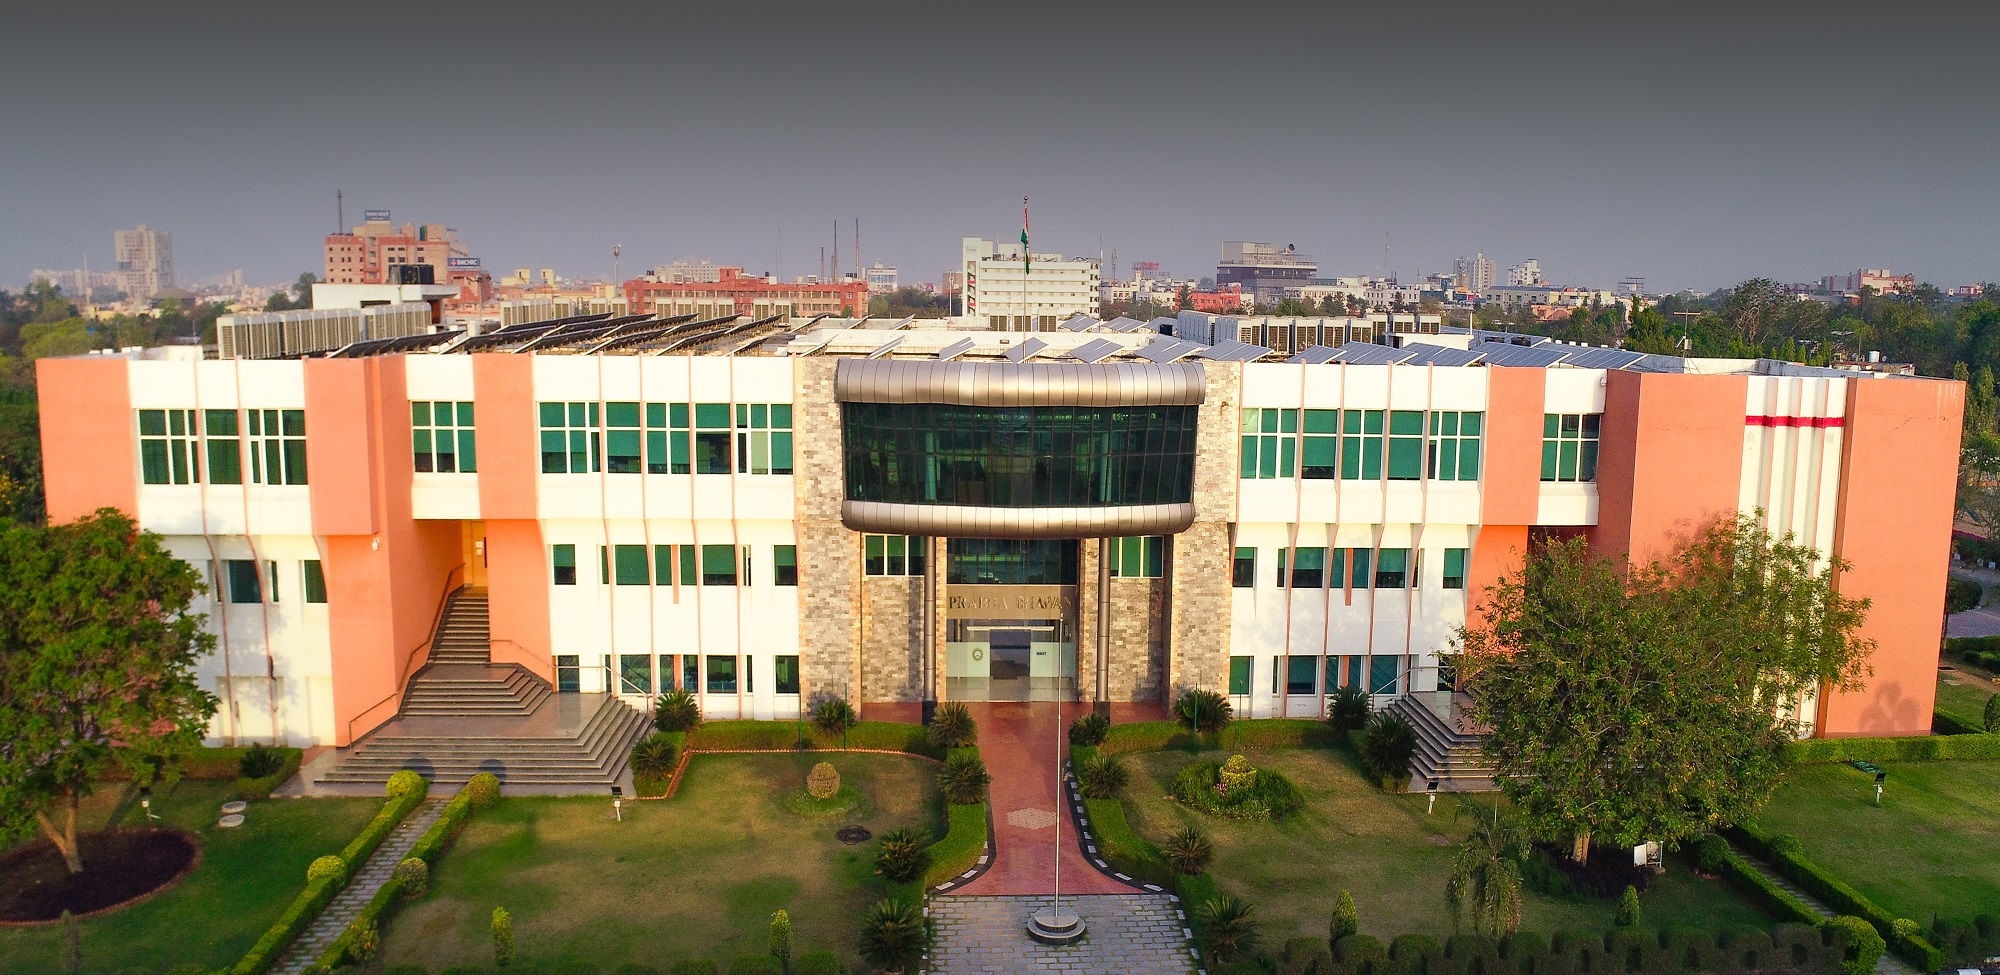
\includegraphics[
		width=\textwidth,
		trim=0 0 0 2.5cm,
		clip
		]{prabha_bhawan.jpg}
		
		\caption{This is a floating image and can appear anywhere.}
	\end{figure}
	
	
	\subsection{Multiple images}
	
	This subsection includes two minipages with equal width.
	
	\begin{center}
		
		\begin{minipage}{0.45\textwidth}
			\centering
			
			
\includegraphics[
			width=\linewidth
			]{Mnit_logo.png}
			
			Figure 3: This is the first minipage.
			
		\end{minipage}
		\hfill
		\begin{minipage}{0.45\textwidth}
			\centering
			
			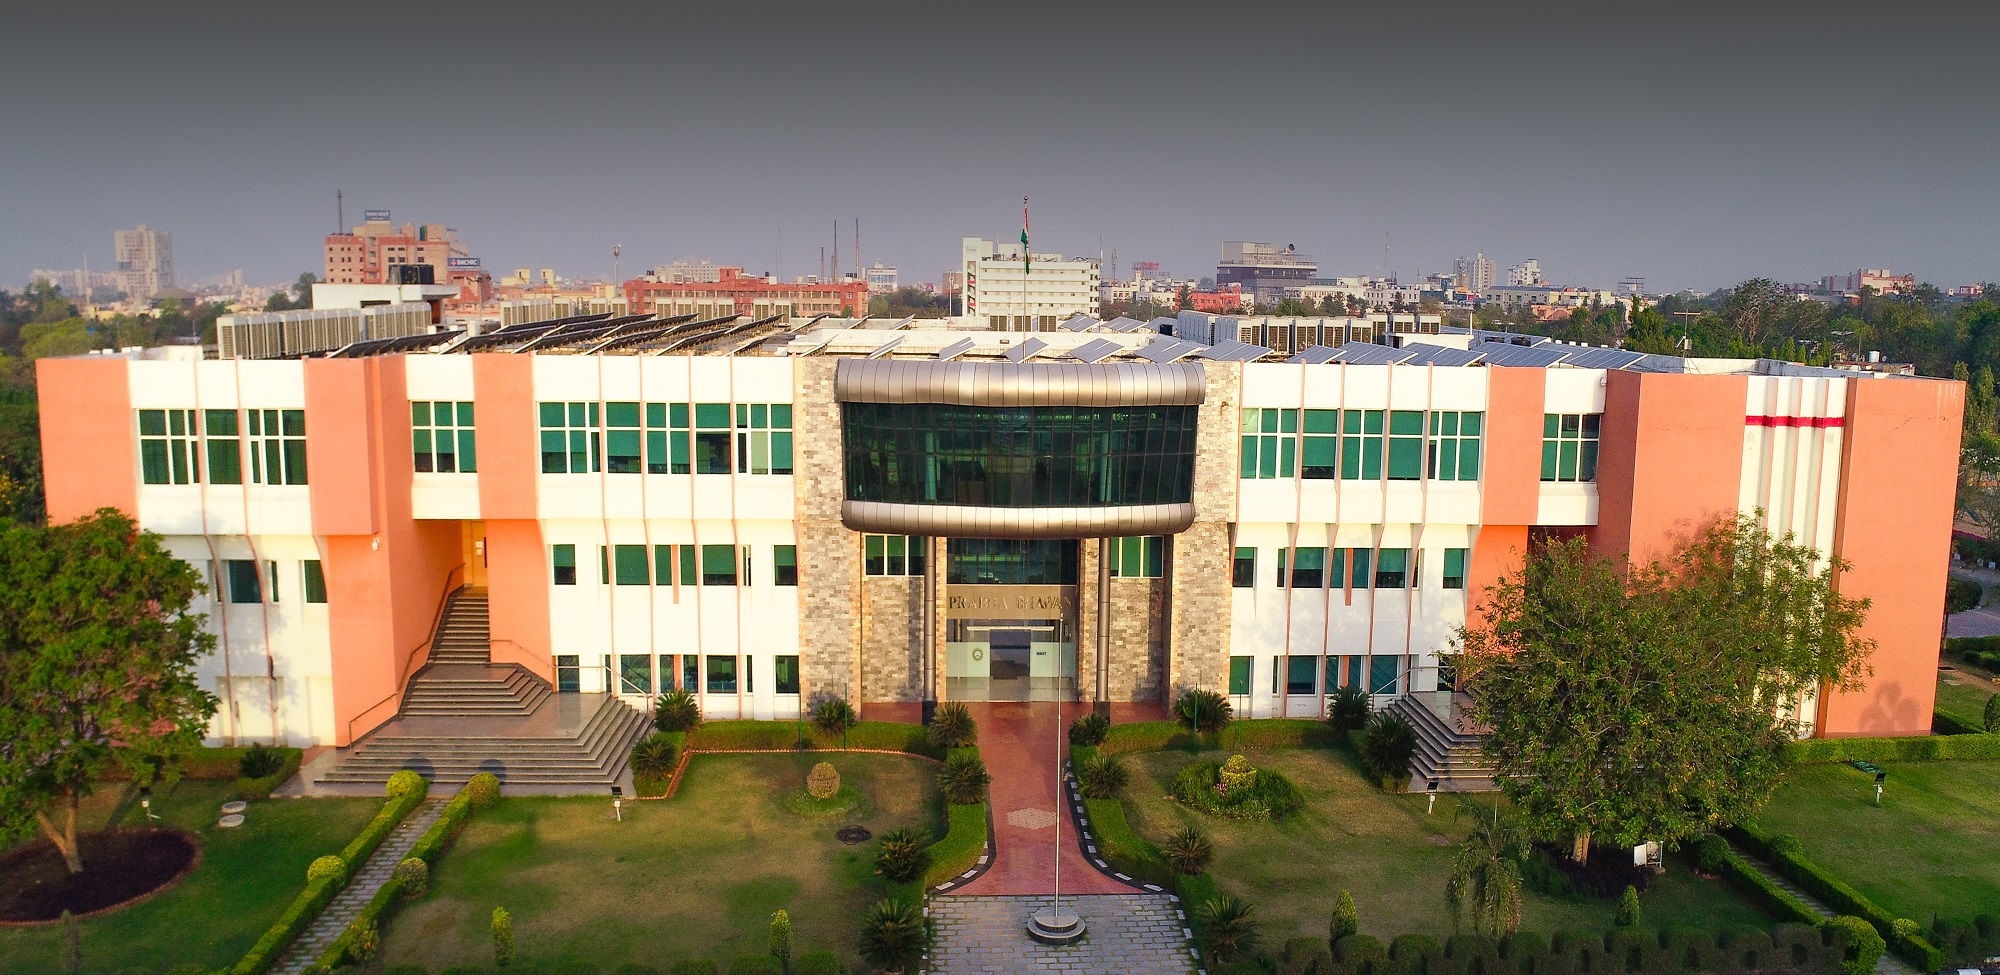
\includegraphics[
			width=\linewidth
			]{prabha_bhawan.jpg}
			
			Figure 4: This is the second minipage.
			
		\end{minipage}
		
	\end{center}
	
	\clearpage
	
	\begin{table}[p]
		\centering
		
		\begin{tabular}{|
				p{2.5cm}|
				p{2cm}|
				p{2cm}|
				p{3.5cm}|
			}
			\hline
			
			\rowcolor{green}
			Language &
			Requires compilation &
			Output &
			Use \\
			
			\hline
			
			C/C++ &
			Yes &
			Executable &
			To make apps \\
			
			\hline
			
			\LaTeX &
			Yes &
			PDF &
			To make documents \\
			
			\hline
			
			HTML/CSS/JS &
			No &
			Webpage &
			To make websites \\
			
			\hline
			
			\rowcolor{yellow}
			2.5 cm &
			2 cm &
			2 cm &
			3.5 cm \\
			
			\hline
		\end{tabular}
		
		\caption{This table should be rendered on a special page.}
	\end{table}
	
\end{document}